% This is samplepaper.tex, a sample chapter demonstrating the
% LLNCS macro package for Springer Computer Science proceedings;
% Version 2.20 of 2017/10/04
%
\documentclass[runningheads]{llncs}
%
%
\usepackage{graphicx}
% Used for displaying a sample figure. If possible, figure files should
% be included in EPS format.
%
% If you use the hyperref package, please uncomment the following line
% to display URLs in blue roman font according to Springer's eBook style:
% \renewcommand\UrlFont{\color{blue}\rmfamily}

\DeclareUnicodeCharacter{2212}{-}
\DeclareUnicodeCharacter{22C5}{-}

\begin{document}
%
\title{A novel distributed nature-inspired algorithm for solving optimization problems\thanks{Supported by TECNOLÓGICO NACIONAL DE MÉXICO (TecNM).}}
% (Biological) Life-Cycle Algorithm: A novel distributed nature-inspired algorithm for solving optimization problems
%
\titlerunning{Life-Cycle Algorithm}
% If the paper title is too long for the running head, you can set
% an abbreviated paper title here
%
\author{J. C. Felix-Saul \inst{1} \and
Mario García Valdez\inst{1} \and
Juan J. Merelo Guervós\inst{2}}
%
\authorrunning{F. Author et al.}
% First names are abbreviated in the running head.
% If there are more than two authors, 'et al.' is used.
%
\institute{Department of Graduate Studies, Tijuana Institute of Technology, Tijuana, Mexico \and
Department of Computer Architecture and Technology, Universidad de Granada, Granada, Spain}
%
\maketitle              % typeset the header of the contribution
%
\begin{abstract}
%The abstract should briefly summarize the contents of the paper in 150--250 words.

Several bio-inspired algorithms use population evolution as analogies of
na-ture. In this paper, we present an algorithm inspired by the biological
Life-Cycle of animal species, which consists of several stages: birth, growth,
re-production, and death. As in nature, we intend to execute all these stages
in parallel and asynchronously on a population that evolves constantly. From
the ground up, we designed the algorithm as a cloud-native solution using the
cloud available resources to divide the processing workload, among several
computers or running the algorithm as a cloud service. The algorithm works
concurrently and asynchronously on a constantly evolving population, using
different computers (or containers) independently, eliminating waiting times
between processes. This algorithm seeks to imitate the natural life cycle,
where new individuals are born at any moment and mature over time, where they
age and suffer mutations throughout their lives. In reproduction, couples match
by mutual attraction, where they may have offspring. Death can happen to
everyone: from a newborn to an aged adult, where the individual's fitness will
impact their longevity. As a proof-of-concept, we implemented the algo-rithm
with Docker containers by solving the OneMax problem comparing it with a basic
(sequential) GA algorithm, where it showed favorable and prom-ising results.

\keywords{Distributed Bioinspired Algorithms  \and Genetic Algorithms \and Cloud Computing.}
\end{abstract}

\section{Introduction} 

Bio-inspired algorithms have been very successful when used to solve complex
optimization problems, but as their complexity increases so does the computing
power required. One strategy to address this processing need is to use
distributed computing, or the resources available in the cloud to help find the
solution. This strategy gives us elasticity to adjust (increase or reduce) the
computing power to achieve a balance according to the nature of the problem.

One of the problems that we have identified in this research is that most
bio-inspired algorithms are designed with a traditionally sequential
perspective, where each process must wait for the previous task to finish
before continuing. Some architectures address this issue, what distinguishes
us, is that our proposal presents an algorithm designed in its entirety as a
native solution in the cloud, fully distributed, where its processes are
executed in parallel and asynchronously. This technique makes it easy to scale
the computing power according to the complexity required by the problem.

We designed our algorithm using observation, analysis, and abstraction in
nature to identify what most species in the animal kingdom have in common,
where individuals of a population that best adapt to the environment have
greater chances of survival, reproduction, and improvement of the species.
Imagining as if the task of writing these rules of evolution was in our hands,
questioning how we could solve it?

Like nature, we identified what most species have in common in the life cycle.
Our algorithm works on a constantly evolving population, experiencing the
stages that all living beings undergo: being born, growing up, reproducing, and
dying, where each of these stages will be processes (of our algorithm) that
randomly affect the population individuals, emulating the organic way.

In this research, we seek to demonstrate that it is possible to evolve a
population of individuals, similar to a Genetic Algorithm (GA), using a
distributed, parallel, and asynchronous methodology.

\section{Description of the sections of the Paper} 

\section{State of the art}

Multiple citations are grouped \cite{valdez2021container,krejca2020lower,witt2019upper,merelo2016nodio,merelo2016performance,fortin2012deap,stanley2002evolving}.

% For citations of references, we prefer the use of square brackets
% and consecutive numbers. Citations using labels or the author/year
% convention are also acceptable. The following bibliography provides
% a sample reference list with entries for journal
% articles~\cite{ref_article1}, an LNCS chapter~\cite{ref_lncs1}, a
% book~\cite{ref_book1}, proceedings without editors~\cite{ref_proc1},
% and a homepage~\cite{ref_url1}. Multiple citations are grouped
% \cite{ref_article1,ref_lncs1,ref_book1},
% \cite{ref_article1,ref_book1,ref_proc1,ref_url1}.

\subsection{Background}

One of the publications with the most influence on our research proposes a
cloud-native optimization framework, that can include multiple
(population-based) algorithms~\cite{valdez2021container}. In their research, they work with ideas such
as those mentioned in Fig.~\ref{fig1}.

\begin{figure}
    \centering
    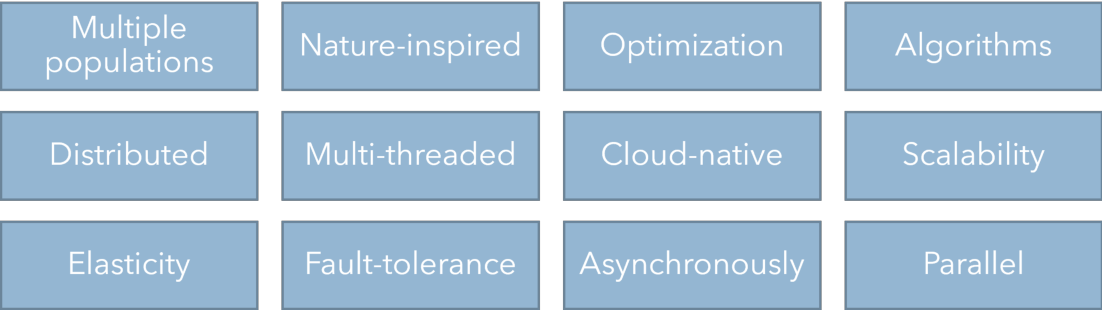
\includegraphics[width=80mm]{img/fig1_background.pdf}
    \caption{These ideas planted the seed of thought in our current presentation.} \label{fig1}
    \end{figure}

\section{Proposal} 

In this paper, we present an algorithm inspired by the biological Life-Cycle of
animal species, which consists of several stages: birth, growth, reproduction,
and death. As in nature, we intend to execute all these stages in parallel and
asynchronously on a population that evolves constantly.

From the ground up, we designed the algorithm as a cloud-native solution using
the cloud available resources to divide the processing workload, among several
computers or running the algorithm as a cloud service. The algorithm works
concurrently and asynchronously on a constantly evolving population, using
different computers (or containers) independently, theoretically eliminating
waiting times between processes.

This algorithm seeks to imitate the natural life cycle, where new individuals
are born at any moment and mature over time, where they age and suffer
mutations throughout their lives. In reproduction, couples match by mutual
attraction, where they may have offspring. Death can happen to everyone: from a
newborn to an aged adult, where the individual's fitness will impact their
longevity. The general model concept is shown on the Fig.~\ref{fig2}.

\begin{figure}
    \centering
    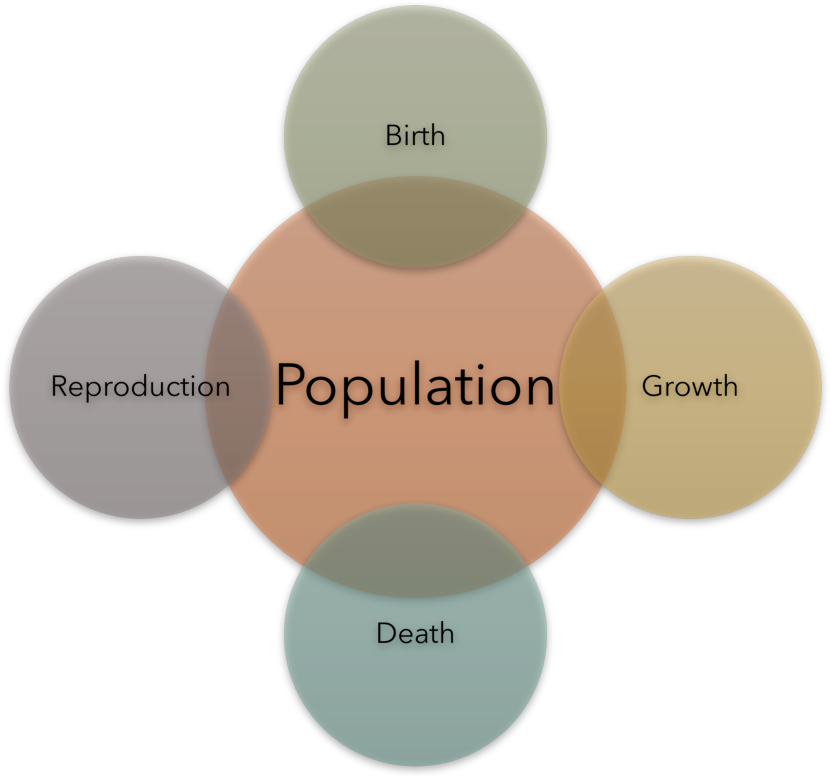
\includegraphics[width=70mm]{img/fig2_proposal.pdf}
    \caption{Algorithm model inspired by the animal species' biological Life-Cycle.} \label{fig2}
    \end{figure}

\subsection{Birth}

This algorithm starts with a randomly generated population, where the processes
will interact with the population independently. This means that at any given
time, any individual can experience any of these processes. Birth is the first
process of our algorithm, and it is responsible for the initial generation of
individuals.

\subsection{Growth}

As in nature, all individuals constantly grow, mature, or age. With increasing
age, individuals may lose strength but also gain more knowledge to solve
problems. We represent this with a possible mutation in each increment of age.
The growth process will take an individual to assess whether it's ready to
mature and undergo changes.

\subsection{Reproduction}

The attraction of a couple will depend on fitness: the better individual's
fitness, the more attractive it will be, making it easier to find mating
matches. This process will be taking random pairs of individuals to evaluate
their attraction as a couple, to try to breed; when the gestation is
successful, a new pair of individuals will be born (as the offspring). Not all
couples will be compatible, so reproduction will not always be possible, but
the problem arises: how to quantify the attraction between two individuals?

We could have used several strategies to evaluate this attraction. Considering
this algorithm takes a similar focus as the study of bacteria growth in
microbiology, where we can observe and analyze the evolution of a population
over time. As in nature' most species, the bigger a specimen is, the more
attractive it is to its mating candidates. To be consistent with both ideas in
our algorithm, we use the equation of Newton's Law of Universal Gravitation (1)
to calculate the attraction between two individuals, where we visualize the
individual fitness as its mass when using the equation. In previous work,
Newton's Law of Universal Gravitation has shown success in helping to solve
optimization problems.

\begin{figure}
    \centering
    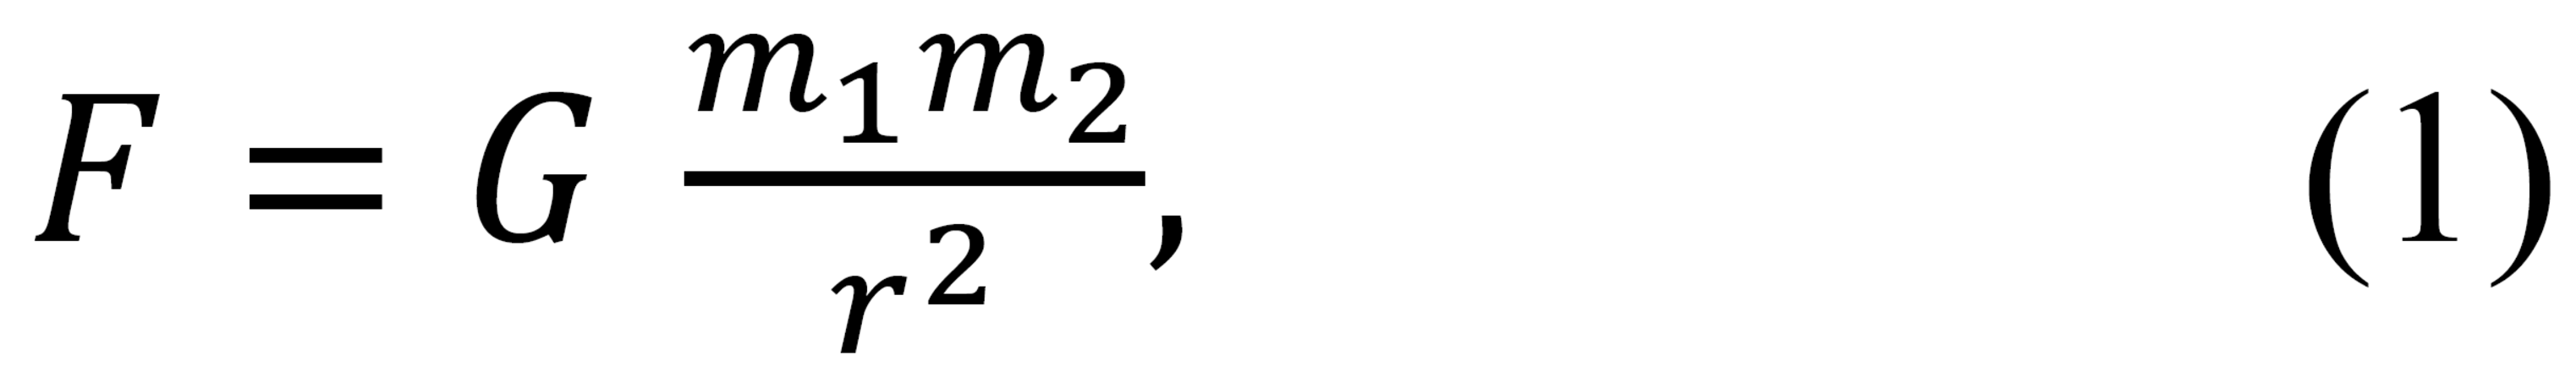
\includegraphics[width=50mm]{img/fig3_newtonslaw.pdf}
    \caption{Newton's Law of Universal Gravitation.} \label{fig3}
    \end{figure}

Where:
\begin{description}  % When enumerating with description, bullet alternatives: cdot, bullet, ast
    \item[$\bullet$ F] is the gravitational force acting between two objects
    \item[$\bullet$ m1 and m2] are the masses of the objects
    \item[$\bullet$ r]	is the distance between the centers of their masses
    \item[$\bullet$ G]	is the gravitational constant: 6.67430(15)×10−11 m3⋅kg−1⋅s−2
\end{description}


\subsection{Death}

The death stage represents the challenges and adversities that life presents to
overcome. This process evaluates the individual resistance to survive in the
environment. The better fitness the individual has will increase its chances of
survival. As time progresses, the demands of nature will also increase, pushing
for only the best individuals to survive.

\subsection{Life-Cycle algorithm flowchart}

The Figure~\ref{fig4} describes the general flowchart for the Life-Cycle algorithm.

\begin{figure}
    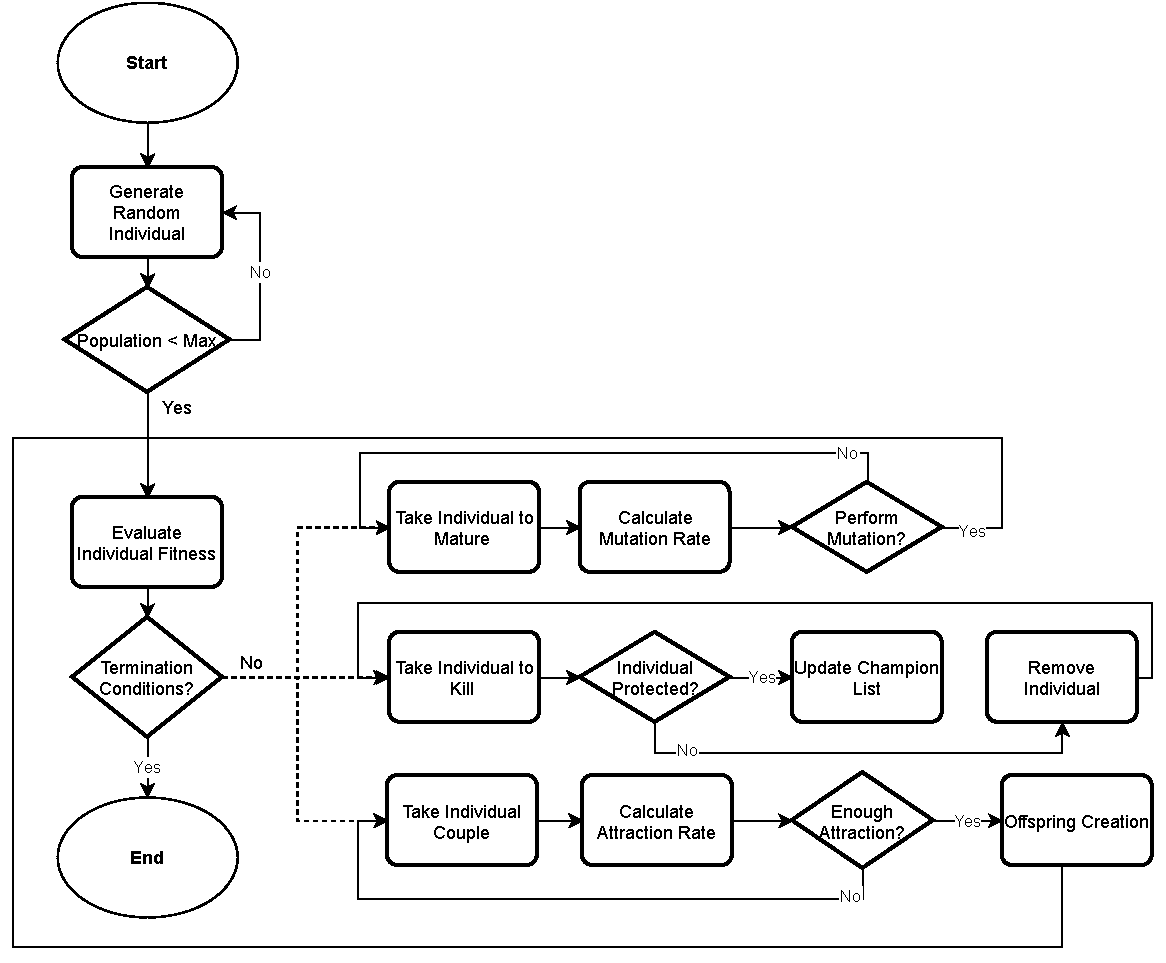
\includegraphics[width=\textwidth]{img/fig4_flowchart.pdf}
    \caption{Life-Cycle algorithm general flowchart.} \label{fig4}
    \end{figure}


\section{Experiments} 

As a proof-of-concept, we implemented the algorithm with Docker containers by
solving the OneMax problem to compare it with a traditional GA algorithm using
the DEAP (Distributed Evolutionary Algorithms in Python) library. The OneMax
problem uses a genetic algorithm to evolve a population of randomly generated
individuals with zeros and ones, and it stops until a solution of only ones is
found.

\subsection{Experimental Setup}

\begin{figure}
    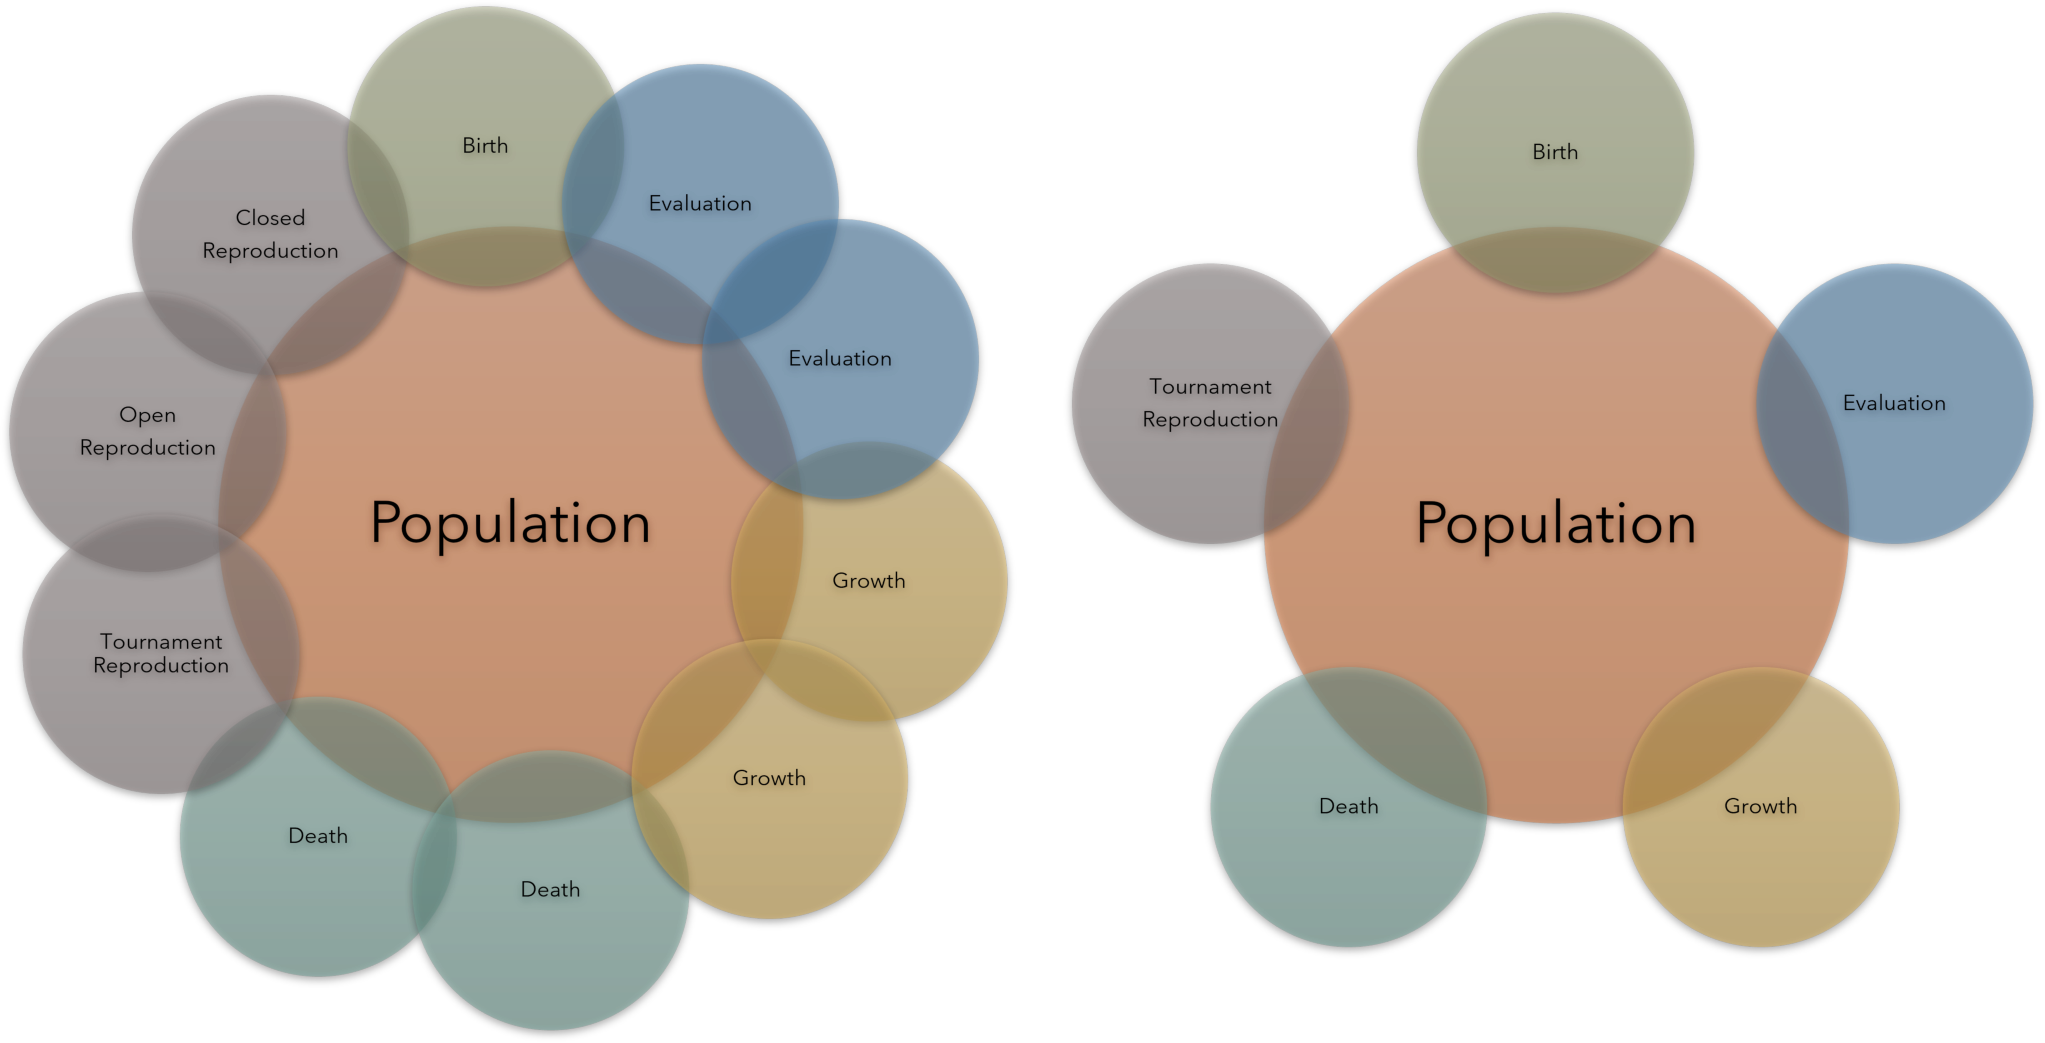
\includegraphics[width=\textwidth]{img/fig5_processes_containers.pdf}
    \caption{Life-Cycle algorithm processes in containers comparison.} \label{fig5}
    \end{figure}

One strategic difference in our algorithm implementation is the reproduction
process, which is flexible to work in parallel with multiple couple selection
methods, for example, tournament selection, random selection (closed
reproduction), and couple match by creating a new mating individual (open
reproduction). We use many combinations of the containerized processes, up to
the minimum number required to obtain good results. Figure~\ref{fig5} shows a comparison
of only two alternatives for the implementation of the algorithm. Our
experimentation started with a configuration of ten processes and ended in
five, shown on the left and right sides of Fig.~\ref{fig5}, respectively.

\subsection{Experiment Configuration}

In this experiment, we needed to match or balance the experimentation
parameters according to the specifications of the algorithm used by the DEAP
library. This is to be able to verify if our algorithm would also converge on
the solutions in a similar number of evaluations and execution time.
Table~\ref{tab1} shows the OneMax initial configuration for DEAP and Life-Cycle
experiment.

\begin{table}[]
    \centering        
    \caption{OneMax initial configuration for DEAP and Life-Cycle experiment.}\label{tab1}
    \begin{tabular}{|l|l|l|}
    \hline
    \textbf{Configuration} & \textbf{DEAP} & \textbf{Life-Cycle} \\ \hline
    Population & 60 & 60 \\ \hline
    Max Generation & 20 & 20 \\ \hline
    Stagnation & Off & 10 \\ \hline
    Chromosome Length & 20 & 20 \\ \hline
    Target Fitness & 20 & 20 \\ \hline
    Crossover Rate & 100 & 100 \\ \hline
    Mutation Rate & 7 & 7 \\ \hline
    Tournament Rate & 100 & 50 \\ \hline
    Tournament Sample & 3 & 4 \\ \hline
    Open Reproduction Rate & NA & 5 \\ \hline
    Closed Reproduction Rate & NA & 45 \\ \hline
    Max Age & NA & 80 \\ \hline
    Base Approval & NA & 80 \\ \hline
    Goal Approval & NA & 100 \\ \hline
    \end{tabular}
    \end{table}


\subsection{Experiment Results}

For each experiment, we ran 60 independent executions per algorithm and
recorded the following results: Last Generation, Total Evaluations, Time
(seconds), Evaluations/second. The labels used on the table header are the
following:

\begin{description}  % When enumerating with description, bullet alternatives: cdot, bullet, ast
    \item[$\bullet$ Last Gen.:] The generation that found the solution.
    \item[$\bullet$ Eval.:] The total number of evaluations the algorithm executed. 
    \item[$\bullet$ Time (sec):] Total elapsed or wall clock time, in seconds. 
    \item[$\bullet$ Eval/sec:] The calculated rate of evaluations per second.
\end{description}


Experiment 1: The goal of our first OneMax experiment was to make sure our
Life-Cycle algorithm worked as expected, converging on the solution. For this
experiment, we intentionally used delays (on the tenth of a second magnitude)
to follow the Life-Cycle algorithm behavior on the console output. For this
experiment, we compared the DEAP algorithm versus the Life-Cycle using ten
processes (on containers) where we show the summarized results in Table~\ref{tab2}, and
Figure~\ref{fig6} shows their Box and Whisker chart.

\begin{table}[]
    \centering        
    \caption{Experiment 1 results: OneMax DEAP versus Life-Cycle (10 processes).}\label{tab2}
    \begin{tabular}{|l|l|l|l|l|l|l|l|l|}
    \hline
    Run & \multicolumn{4}{l|}{OneMax DEAP} & \multicolumn{4}{l|}{Life-Cycle (10P)} \\ \hline
    1-60 & Last Gen. & Eval. & Time (sec) & Eval/sec & Last Gen. & Eval. & Time (sec) & Eval/sec \\ \hline
    Avg. & 6.5 & 391 & 0.036 & 10,836 & 9.6 & 578 & 6.830 & 85 \\ \hline
    \end{tabular}
    \end{table}

\begin{figure}
    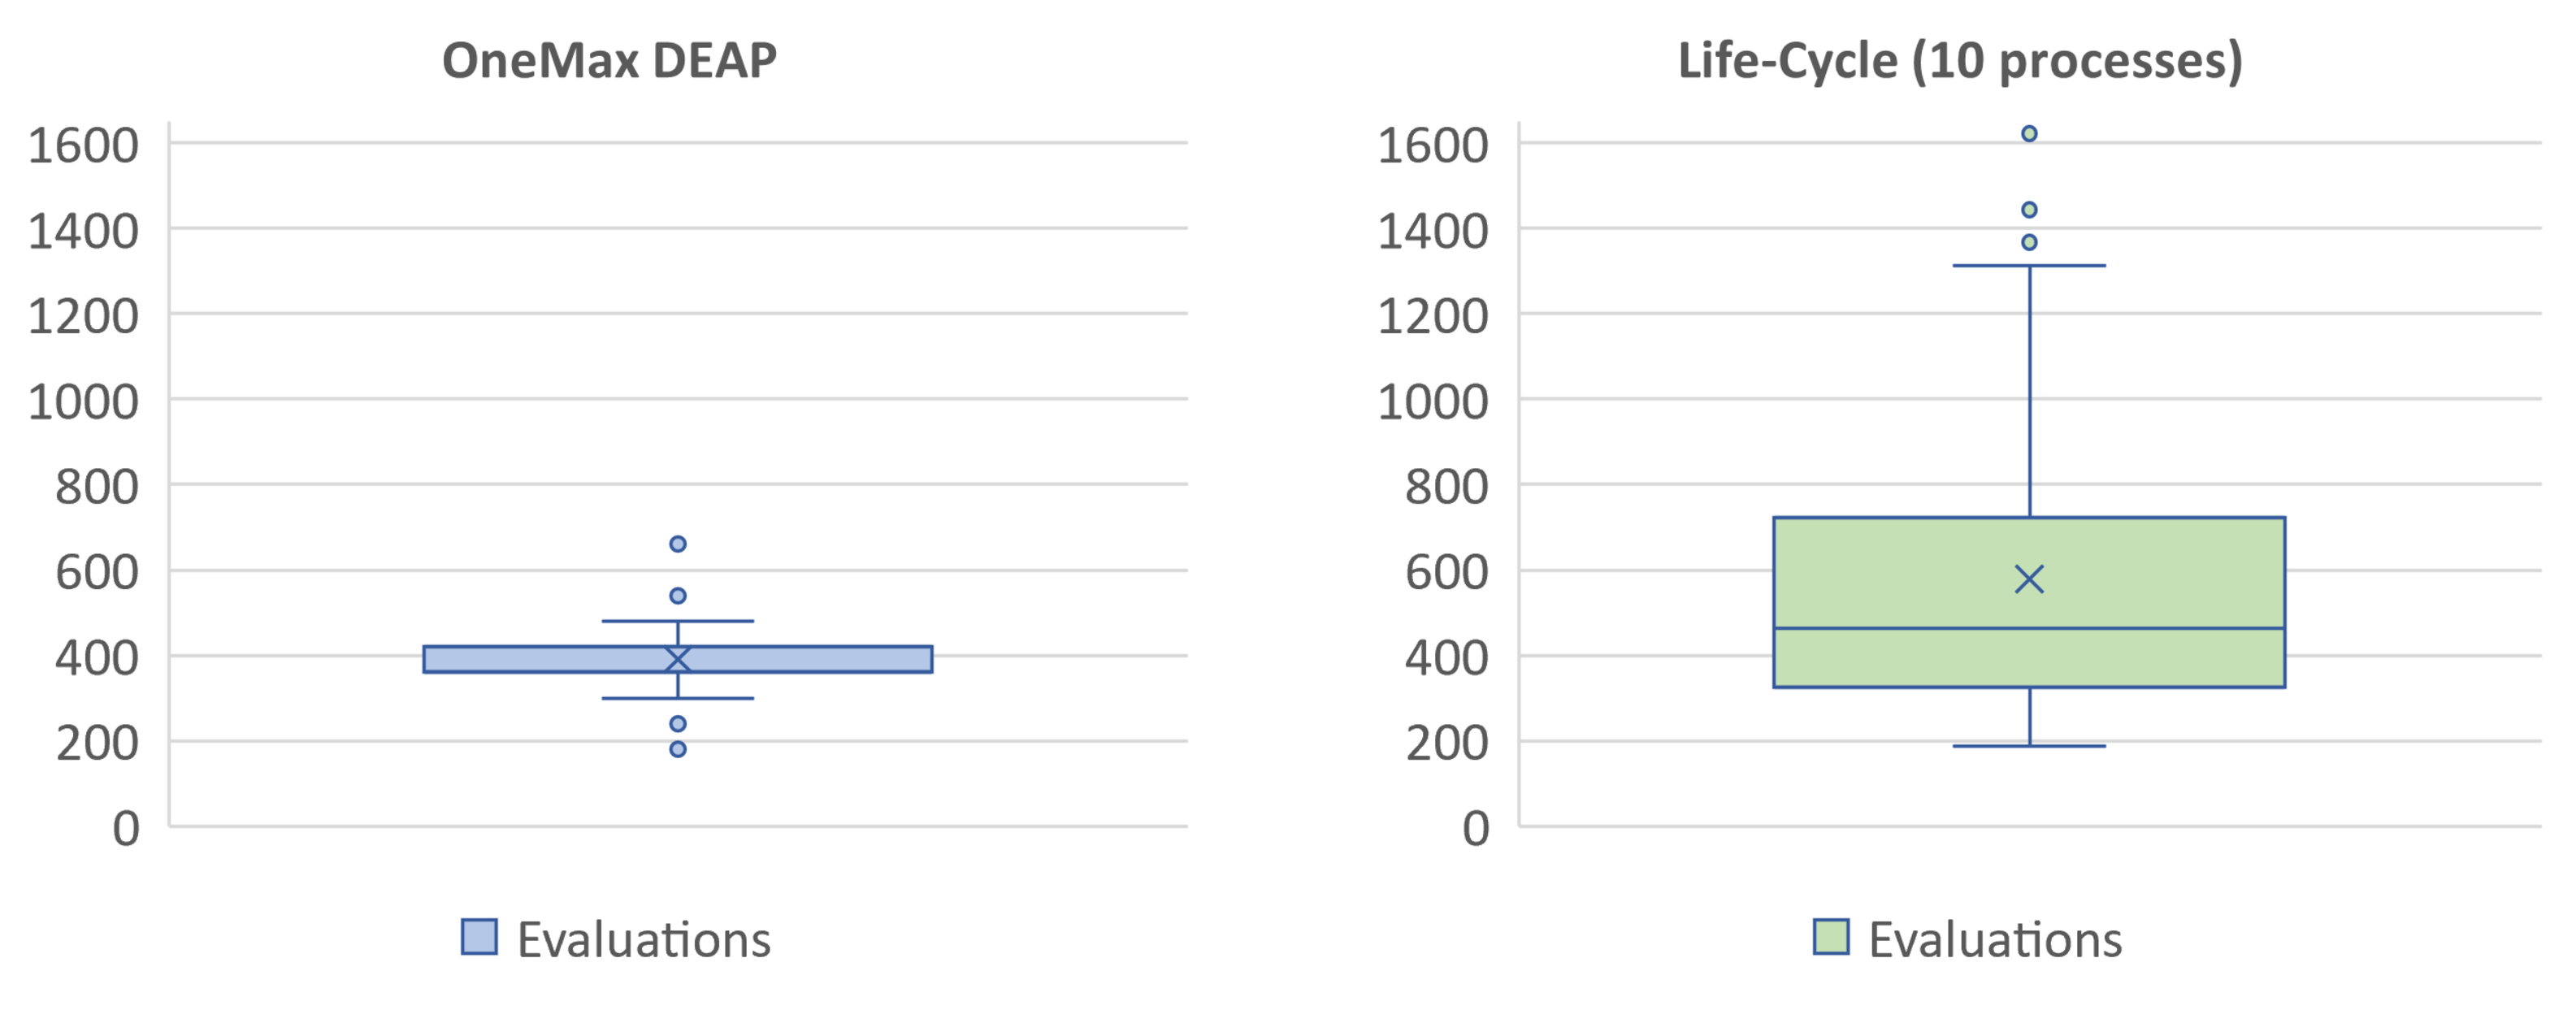
\includegraphics[width=\textwidth]{img/fig6_experiment01_chart.pdf}
    \caption{Box and Whisker chart for the Experiment 1: OneMax DEAP versus Life-Cycle (10 processes).} \label{fig6}
    \end{figure}


Experiment 2: The goal of our second experiment was to confirm the Life-Cycle
algorithm continued working as expected, converging on the solution. For this
experiment, we reduced the time used on delays (now on the thousands of a
second magnitude) to follow the Life-Cycle algorithm behavior. For this
experiment, we only used tournament selection for the reproduction, on the
first configuration running the Life-Cycle on ten processes, versus the second
configuration where we reduced the processes to the minimum basic 5. We show
the summarized results in Table~\ref{tab3}, and Figure~\ref{fig7} shows their Box and Whisker
chart.

\begin{table}[]
    \centering        
    \caption{Experiment 2 results, Life-Cycle Tournament selection: 10 versus 5 processes.}\label{tab3}
    \begin{tabular}{|l|l|l|l|l|l|l|l|l|}
    \hline
    Run & \multicolumn{4}{l|}{LifeCycle (Tourn. 10P)} & \multicolumn{4}{l|}{LifeCycle (Tourn. 5P)} \\ \hline
    1-60 & Last Gen. & Eval. & Time (sec) & Eval/sec & Last Gen. & Eval. & Time (sec) & Eval/sec \\ \hline
    Avg. & 7.2 & 434 & 0.740 & 587 & 8.2 & 495 & 0.826 & 599 \\ \hline
    \end{tabular}
    \end{table}

\begin{figure}
    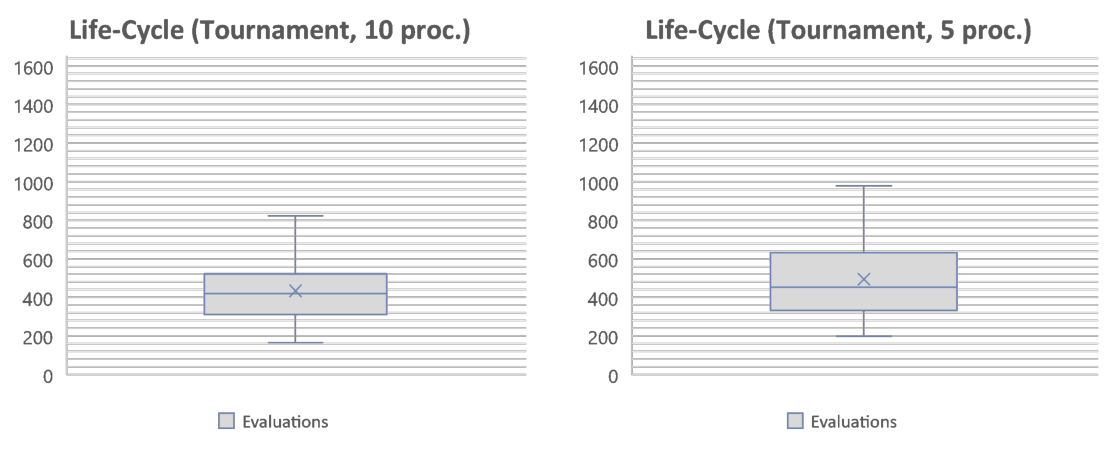
\includegraphics[width=\textwidth]{img/fig7_experiment02_chart.pdf}
    \caption{Box and Whisker chart for the Experiment 2: Life-Cycle Tournament selection (10 versus 5 processes).} \label{fig7}
    \end{figure}


Experiment 3: The goal of our third experiment was to follow and study the
behavior of the Life-Cycle algorithm that continued converging on the solution.
For this experiment, we remained using minimal delays (thousands of a second
magnitude). For this experiment, we only used tournament selection for the
reproduction, on the first configuration running the Life-Cycle on six
processes, two of whom was the Death stage, versus the second configuration
where we reduced the processes to the minimum (five) but increasing the (Death)
goal approval range to 115. We show the summarized results in Table~\ref{tab4}, and
Figure~\ref{fig8} shows their Box and Whisker chart.

\begin{table}[]
    \centering        
    \caption{Experiment 3 results, Life-Cycle Tournament: 6 processes (Death x2) versus 5 processes (80 to 115 goal).}\label{tab4}
    \begin{tabular}{|l|l|l|l|l|l|l|l|l|}
    \hline
    Run & \multicolumn{4}{l|}{LifeCycle (Tourn. 6P, Death x2)} & \multicolumn{4}{l|}{LifeCycle (Tourn. 5P, 80-115g)} \\ \hline
    1-60 & Last Gen. & Eval. & Time (sec) & Eval/sec & Last Gen. & Eval. & Time (sec) & Eval/sec \\ \hline
    Avg. & 8.0 & 483 & 0.846 & 571 & 6.4 & 384 & 0.695 & 553 \\ \hline
    \end{tabular}
    \end{table}

\begin{figure}
    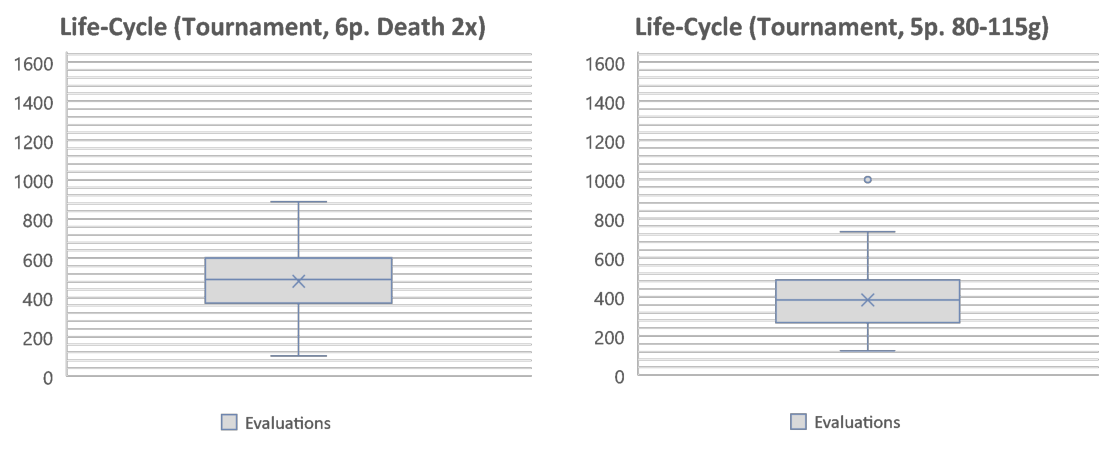
\includegraphics[width=\textwidth]{img/fig8_experiment03_chart.pdf}
    \caption{Box and Whisker chart for the Experiment 3: Life-Cycle Tournament (6 proc. Death x2, versus 5 proc. w/115 goal).} \label{fig8}
    \end{figure}


Experiment 4: The goal of our fourth and last experiment was to follow and
study the behavior of the Life-Cycle algorithm that continued converging on the
solution. For this experiment, we remained using minimal delays (thousands of a
second magnitude). For this experiment, we compared the OneMax DEAP
implementation versus the Life-Cycle algorithm, only using tournament selection
for the reproduction, with the Life-Cycle configuration running on the minimum
(five) processes but increasing the (Death) goal approval range to 125. We show
the summarized results in Table~\ref{tab5}, and Figure~\ref{fig9} shows their Box and Whisker
chart.

\begin{table}[]
    \centering        
    \caption{Experiment 4 results, OneMax DEAP versus Life-Cycle Tournament: 5 processes (80 to 125 goal).}\label{tab5}
    \begin{tabular}{|l|l|l|l|l|l|l|l|l|}
    \hline
    Run & \multicolumn{4}{l|}{OneMax DEAP} & \multicolumn{4}{l|}{Life-Cycle (Tourn. 5P, 80-125g)} \\ \hline
    1-60 & Last Gen. & Eval. & Time (sec) & Eval/sec & Last Gen. & Eval. & Time (sec) & Eval/sec \\ \hline
    Avg. & 6.5 & 391 & 0.036 & 10,836 & 6.3 & 377 & 0.678 & 556 \\ \hline
    \end{tabular}
    \end{table}

\begin{figure}
    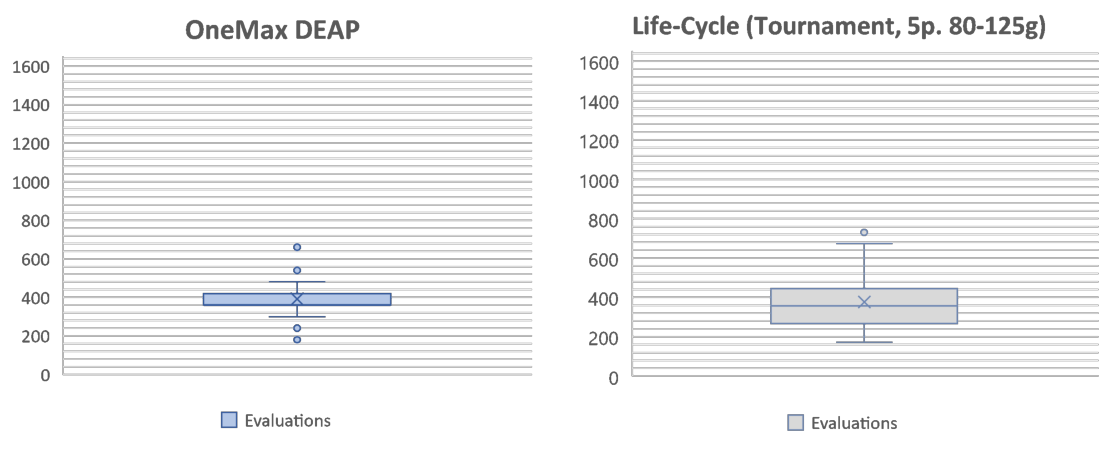
\includegraphics[width=\textwidth]{img/fig9_experiment4_chart.pdf}
    \caption{Box and Whisker chart for the Experiment 4: OneMax DEAP versus Life-Cycle Tournament (5 proc. w/125 goal).} \label{fig9}
    \end{figure}

% Table~\ref{tab3} shows the OneMax DEAP experiment results, while Table~\ref{tab4} shows the LifeCycle Algorithm experiment results.


\section{Discussion}

In our experiments, we found that for simple problems, the cost of
communication between containers will increase the total time of execution,
however, we believe that the opposite must also be true: for complex problems,
distributing the work on multiple resources must reduce time, making the
communication cost negligible.

This scheme allows for multiple parameter's fine tunning, granting us the
freedom to experiment with different selection and reproduction strategies
simultaneously, which will impact how fast it finds the solution and the
obtained quality.

\section{Conclusions}

We implemented the algorithm with Docker containers by solving the OneMax
problem comparing it with a traditional (sequential) GA algorithm, where it
showed favorable and promising results. To further validate this work, we could
use control or some more complex and demanding problem that requires computing
real numbers.

As the complexity of problems increases, it is essential to have a scalable,
replicable, and fault-tolerant model that uses collaborative techniques to work
in the cloud, where multiple resources will be communicating asynchronously.
This research has shown that it is possible to evolve a population of
individuals, similar to a Genetic Algorithm (GA), using a distributed,
parallel, and asynchronous methodology.


%
%
%

% Introducción 
% Contexto: Los algoritmos bioinsirados se utilzan para resolver 
% problemas complejos, pero en ocasiones se requiere de poder
% computo.
% Problemas: La mayoría de los algoritmos bio inspiarados
% no están diseñandos con perspectiva distribuida, paralela y asíncrona. 
% De que hay arquitecturas que tratan esta problematica. 
% Propuesta. 
% Descripción de las secciones del paper.

% Estado del Arte 
% PSO distribuido, GAs, etc.

% Propuesta
% 

% Experimental 
% Setup 
% OneMax
% Results 

% Conclusiones

%
% ---- Bibliography ----
%
% BibTeX users should specify bibliography style 'splncs04'.
% References will then be sorted and formatted in the correct style.
%
\bibliographystyle{splncs04}
\bibliography{bib/bibliografia.bib}
%
\end{document}
